\documentclass[twoside,11pt]{article}
\PassOptionsToPackage{longnamesfirst}{natbib}
\usepackage{obs_study_style}
\usepackage{amsmath,booktabs,array}
\usepackage[hidelinks]{hyperref}
\heading{}{}{}{}{}{Yunjie Guo and Hanqing Yang}
\ShortHeadings{Estimand alignment in a four-arm comparison}{Guo and Yang}
\firstpageno{1}
\title{Estimand Alignment in a Four-Arm Within-Study Comparison}
\author{\name Yunjie Guo \\
  \addr Independent Researcher, Suzhou, China
  \AND \name Hanqing Yang \email hanqing.yang189@gmail.com \\
  \addr Independent Researcher, Suzhou, China (corresponding author)}
\date{}

\begin{document}
\maketitle
\thispagestyle{plain}
\shortcites{chernozhukov2018}

\begin{abstract}%
In a four-arm preference study, participants state which intervention they prefer before random assignment. An observational analysis restricted to participants who received their preferred intervention can target a different population from the full trial. We derive a randomized benchmark for this concordant population under any common assignment probability. Its average effect equals the full-population effect when assignment is equally likely or when the two preference groups have equal average effects. We apply the benchmark to a public trial of mathematics and vocabulary training in 2,200 participants. For mathematics, the prespecified observational and randomized estimates among participants who preferred mathematics were 0.794 and 0.795 points. Their difference had a 95\% bootstrap interval of $[-0.95,0.66]$. Of the 0.315-point gap between the observational average effect and the full-sample randomized estimate, only $-0.0002$ points came from the difference in preference composition. For vocabulary, the largest aligned discrepancy was 0.91 points among participants who preferred mathematics. Its marginal interval excluded zero, while its interval adjusted for six exploratory contrasts included zero. In this study, aligning the comparison populations changed the estimated gap little, and the primary interval allowed discrepancies comparable in size to the randomized effect.
\end{abstract}

\begin{keywords}
within-study comparison, estimand alignment, treatment preference, overlap, cross-fitting
\end{keywords}

\section{Introduction}
\label{sec:intro}

Within-study comparisons place a randomized estimate and a nonrandomized estimate in one empirical setting, so that differences of site, intervention, or outcome instrument are less available as explanations for a discrepancy \citep{cook2008,keller2025,wongsteiner2018}. The comparison still has to say which causal parameter each estimate targets. A randomized contrast among people who preferred treatment, an average effect in the subset whose assignment matched their preference, and an average effect in the full sample can all be well defined and still be different parameters. Calling every gap between an observational estimate and a randomized estimate ``bias'' collapses three separate ideas: whether two estimands are the same, whether an observational functional identifies its target, and how precisely either quantity is estimated.

The public four-arm study of \citet{keller2025} makes that distinction concrete. Participants stated a preference for a mathematics or a vocabulary session and were then assigned at random to one of the two sessions. The subset in which assignment matches preference is the concordant population. Inside it, the people assigned to mathematics are exactly the people who preferred mathematics. The design therefore supplies randomized benchmarks for the preference-group effects and for a preference-weighted effect in the concordant population. Those benchmarks are design facts about estimands. They do not justify an observational analysis of the concordant subset that adjusts for covariates: in that subset, treatment and preference are the same variable, so conditional exchangeability is an assumption about self-selection.

\subsection{Related work}

One influential comparison of nonexperimental estimators against an experimental benchmark is the training-program reanalysis of \citet{dehejia1999}. Other designs place the observational and experimental comparisons within a single study. \citet{shadish2008} randomized participants either to random assignment or to self-selection between mathematics and vocabulary training, a design closely related to the two-stage preference trial of \citet{rucker1989}, and found that adjusted self-selection estimates came close to the randomized ones. \citet{steiner2010} analyzed which covariates did the work in that adjustment. \citet{cook2008} summarized the conditions under which observational and experimental estimates agree. Large-sample comparisons with modern estimators, such as the advertising experiments of \citet{gordon2019}, report less favorable agreement.

Two strands bear directly on this paper. The first concerns estimands in preference designs. \citet{long2008} and \citet{marcus2012} treat preference as a pretreatment stratum and define causal effects within preference groups and effects of being allowed to choose. \citet{keller2025} replace the first-stage randomization of \citet{shadish2008} by a design in which everyone states a preference and everyone is randomized, and they show that the observational effects on the treated and on the untreated in the concordant subset are randomized-trial parameters. Our Proposition~\ref{prop:concordant} is an elementary consequence of the same design. We state it because it isolates exactly when the full-sample average treatment effect is a valid benchmark for a concordant observational average effect, and because it yields a finite-sample decomposition that can be computed. The second strand concerns how correspondence should be judged. \citet{steinerwong2018} examine distance-based criteria and recommend combining significance and equivalence testing. Our protocol did not fix an equivalence margin, so we report intervals for the discrepancies and make no equivalence claim.

\subsection{Questions and contribution}

This paper asks three questions. First, how can the four-arm design construct a randomized benchmark for the treatment effect in the concordant population? Second, how does that benchmark relate to the average treatment effect in the full population? Third, how should a numerical discrepancy between an observational estimator and a randomized estimator be read when the estimands, the populations, and the estimation procedures are not the same?

The empirical analysis uses the public sample of 2{,}200 participants. The primary comparison, for the mathematics post-test, was specified before those estimates were examined. It pairs the randomized difference in means among mathematics-preferring participants with a cross-fitted augmented inverse-probability-weighted estimator of the average treatment effect on the treated in the concordant subset \citep{bang2005,chernozhukov2018}. The vocabulary post-test was listed as the secondary outcome in the same protocol. We analyze it with the identical specification after reversing the treatment and preference codes, and we wrote that specification down before computing any vocabulary estimate. Cross-fitting seeds, an alternative randomized estimator, covariate subsets, an inverse-probability sensitivity bound, and overlap restrictions are reported as exploratory analyses.

The contribution is interpretive and empirical, not a new estimator. The concordant-population benchmark can be formed for any common assignment probability strictly between zero and one; its equivalence to the full-population average effect still requires assignment probability one half or equal preference-group effects. In the mathematics outcome the primary point estimates nearly agree, while the prespecified interval does not support a claim of recovery, equivalence, or negligible confounding. In the vocabulary outcome every aligned observational estimate exceeds its randomized benchmark, by 0.39 to 0.91 points, and precision varies with the direction of reweighting. In both outcomes estimand composition is negligible in the observed sample for a mechanical reason, and that fact does not identify the observational average effect.

\section{Study design and data}
\label{sec:design}

Let $S\in\{0,1\}$ denote preference for the mathematics session, and let $D\in\{0,1\}$ denote randomized assignment to that session. The concordant population is $C=\{D=S\}$. The four realized cells are G1, $(S,D)=(1,1)$; G2, $(1,0)$; G3, $(0,1)$; and G4, $(0,0)$. Table~\ref{tab:cells} gives the counts in the public file: 288, 319, 776, and 817. Mathematics assignment was realized for $288+776=1{,}064$ participants and vocabulary assignment for $319+817=1{,}136$. The analysis sample is the released WSCdata file of $N=2{,}200$ rows described by \citet{keller2025}. The primary outcome is the mathematics post-test, \texttt{mathPost}. The secondary outcome is the vocabulary post-test, \texttt{vocabPost}; its standard deviation is 4.10 points, against 3.56 for \texttt{mathPost}.

\begin{table}[htbp]
\centering
\caption{Realized four-arm cells. $S$ is preference for mathematics and $D$ is assignment to mathematics.}
\label{tab:cells}
\begin{tabular}{llrr}
\toprule
Cell & Definition & Role in $C=\{D=S\}$ & $n$ \\
\midrule
G1 & $S=1$, $D=1$ & Concordant, assigned mathematics & 288 \\
G2 & $S=1$, $D=0$ & Discordant & 319 \\
G3 & $S=0$, $D=1$ & Discordant & 776 \\
G4 & $S=0$, $D=0$ & Concordant, assigned vocabulary & 817 \\
\bottomrule
\end{tabular}
\end{table}

Under the published description of the WSC randomization design, preference was elicited before assignment, and assignment was then made regardless of preference \citep{keller2025}. The same description states that assignment was completely at random with probability one half and writes the assignment indicator as independent of preference and of the two potential outcomes. It does not describe stratification or blocking on preference. We did not inspect the assignment program. The package documentation identifies the randomized indicator and the four-arm coding; it does not state the assignment probability. The realized split $1{,}064/2{,}200$ is compatible with independent assignment at probability one half and is not evidence that the design probability differed from one half.

For \texttt{mathPost}, the primary randomized contrast uses G1 and G2, the two cells with $S=1$, and the primary observational contrast uses the concordant subset G1$\cup$G4 of $1{,}105$ participants. The full-sample randomized difference in means uses all four cells. The preference-group effect for $S=0$ uses G3 and G4. For \texttt{vocabPost}, the treatment of interest is vocabulary training, $1-D$, and the relevant preference is $1-S$. The roles of the cells are then exchanged: the treated concordant cell is G4, the randomized contrast for vocabulary-preferring participants is G4 against G3, and the concordant subset is the same 1{,}105 participants.

\section{Causal estimands}
\label{sec:theory}

Let $Y(1)$ and $Y(0)$ denote the potential post-test outcomes under assignment to the treatment session and to the other session. The preference-group effects, the full-population average treatment effect, and the concordant-population effect are
\begin{align*}
\tau_s &= E[Y(1)-Y(0)\mid S=s], \qquad s\in\{0,1\},\\
\tau_{\mathrm{full}} &= E[Y(1)-Y(0)],\\
\tau_C &= E[Y(1)-Y(0)\mid C].
\end{align*}
Write $p=P(D=1)$, $\pi=P(S=1)$, and $\pi_c=P(S=1\mid C)$. The average treatment effect on the treated in the usual selection sense is $E[Y(1)-Y(0)\mid S=1]=\tau_1$, because the people who prefer the treatment session are the people who would be treated under self-selection. Likewise $\tau_0$ is the average treatment effect on the untreated. The development is written for mathematics as the treatment; for the vocabulary outcome every statement holds after $D$ and $S$ are replaced by $1-D$ and $1-S$.

The design assumptions used for the population identities are the following.

\begin{enumerate}
\item \textbf{Random assignment.} $D\perp\bigl(S,Y(1),Y(0)\bigr)$, with a common assignment probability $0<p<1$ in both preference groups.
\item \textbf{Both preferences occur.} $0<\pi<1$.
\item \textbf{Consistency and no interference.} The observed outcome equals the potential outcome under the realized assignment; there is one treatment version; and one participant's assignment does not change another's potential outcomes. The further statement that randomized assignment and self-selection implement the same treatment version is part of this assumption. It is not implied by independence of $D$.
\end{enumerate}

Assumption~1 is the content of the published randomization description. Assumption~3 is stated separately by \citet{keller2025} and is retained here as an assumption; the preference-trial literature exists precisely because receiving a chosen treatment may differ from receiving the same treatment by lot \citep{rucker1989,marcus2012}. The identities in Proposition~\ref{prop:concordant} use Assumptions~1 and~2. They are statements about potential-outcome estimands. Consistency connects those estimands to contrasts of observed outcomes.

\begin{proposition}
\label{prop:concordant}
Under Assumptions~1 and~2,
\begin{align}
\pi_c
&=
\frac{\pi p}{\pi p+(1-\pi)(1-p)},
\label{eq:pic}\\
E[Y(1)-Y(0)\mid D=1,\,C]
&=
\tau_1,
\label{eq:att}\\
E[Y(1)-Y(0)\mid D=0,\,C]
&=
\tau_0,
\label{eq:atu}\\
\tau_C
&=
\pi_c\tau_1+(1-\pi_c)\tau_0,
\label{eq:tauc}\\
\tau_C-\tau_{\mathrm{full}}
&=
(\pi_c-\pi)(\tau_1-\tau_0).
\label{eq:gap}
\end{align}
Consequently,
\begin{equation}
\tau_C=\tau_{\mathrm{full}}
\quad\Longleftrightarrow\quad
p=\tfrac12
\quad\text{or}\quad
\tau_1=\tau_0.
\label{eq:iff}
\end{equation}
\end{proposition}

\begin{proof}
Independence of $D$ and $S$ gives $P(S=1,D=1)=\pi p$ and $P(S=0,D=0)=(1-\pi)(1-p)$. The event $C$ is the disjoint union of these two cells, so \eqref{eq:pic} is the definition of $\pi_c$. The event $\{D=1\}\cap C$ equals $\{D=1,S=1\}$. Independence of $D$ and $(Y(1),Y(0))$ given $S=1$ therefore yields \eqref{eq:att}, and the symmetric argument yields \eqref{eq:atu}. Conditioning further on $S$ inside $C$,
\[
\tau_C
=
E[Y(1)-Y(0)\mid S=1,\,C]\,\pi_c
+
E[Y(1)-Y(0)\mid S=0,\,C]\,(1-\pi_c).
\]
The two conditional expectations are $\tau_1$ and $\tau_0$, which is \eqref{eq:tauc}. The full-population effect has the same two building blocks with weights $(\pi,1-\pi)$,
\[
\tau_{\mathrm{full}}=\pi\tau_1+(1-\pi)\tau_0,
\]
and this decomposition uses only the law of total expectation. Subtracting it from \eqref{eq:tauc} gives \eqref{eq:gap}. Finally,
\[
\pi_c-\pi
=
\frac{\pi(1-\pi)(2p-1)}{\pi p+(1-\pi)(1-p)}.
\]
The denominator is positive under Assumptions~1 and~2, and $\pi(1-\pi)>0$, so $\pi_c=\pi$ if and only if $p=1/2$. Combined with \eqref{eq:gap}, this is \eqref{eq:iff}.
\end{proof}

Equation~\eqref{eq:iff} is a population identity. It does not say that an estimator of $\tau_C$ is close to an estimator of $\tau_{\mathrm{full}}$ in a finite sample, and it does not identify either parameter from an observational likelihood. The concordant benchmark $\tau_C$ can be assembled from $\tau_1$ and $\tau_0$ without first estimating $p$, because a randomized contrast within $S=1$ targets $\tau_1$ and a randomized contrast within $S=0$ targets $\tau_0$ at whatever common $p$ generated the assignment. Replacing $\tau_C$ by $\tau_{\mathrm{full}}$ is the step that uses $p=1/2$ or homogeneity.

For example, consider a trial with two-to-one allocation to treatment in which one third of participants prefer treatment. Equation~\eqref{eq:pic} gives a treated-preference proportion of one half among concordant participants. If the treatment effect averages two points in the treated-preference group and one point in the other group, the full-population effect is $4/3$ points and the concordant effect is $3/2$ points. Comparing a concordant estimator with the full-trial effect would introduce a $1/6$-point gap even if both effects were known exactly. The empirical study below used equal allocation probabilities.

Identification of the same parameters from the observational concordant sample is a different claim. In $C$, the observed treatment indicator is $S$. A covariate-adjusted estimator computed on G1$\cup$G4 therefore identifies $\tau_1$, $\tau_0$, or $\tau_C$ only under additional conditions: conditional exchangeability of preference with the potential outcomes given the covariates, positivity of preference given those covariates, and the treatment-version statement in Assumption~3 \citep{imbens2004}. Randomization of $D$ does not establish conditional exchangeability of $S$. Conditioning on $C$ changes the target population, because $\pi_c$ need not equal $\pi$. It does not create a second treatment version. Whether the randomized session and the session a participant would have self-selected are the same intervention remains an assumption.

\section{Estimation and inference}
\label{sec:estimation}

The randomized building blocks are unadjusted differences in means, with the usual two-sample standard error. Applied to G1 versus G2, the difference in means estimates $\tau_1$. Applied to G3 versus G4, it estimates $\tau_0$. Applied to all $2{,}200$ rows, it estimates the full-sample average effect of assignment. The sample assignment proportion is left as realized. Write $\widehat\tau_1$, $\widehat\tau_0$, and $\widehat\tau^{\mathrm{RCT}}_{\mathrm{full,DM}}$ for these three statistics, and write $\widehat\pi=607/2200$ and $\widehat\pi_c=288/1105$ for the realized preference weight and the realized concordant preference weight. The plug-in benchmarks are
\begin{align*}
\widehat\tau_C
&=
\widehat\pi_c\,\widehat\tau_1+(1-\widehat\pi_c)\,\widehat\tau_0,\\
\widehat\tau_{\mathrm{ps}}
&=
\widehat\pi\,\widehat\tau_1+(1-\widehat\pi)\,\widehat\tau_0.
\end{align*}
The first is the finite-sample concordant benchmark. The second is the preference-post-stratified full-sample benchmark. Their difference equals $(\widehat\pi_c-\widehat\pi)(\widehat\tau_1-\widehat\tau_0)$.

The observational estimator in the concordant subset is a five-fold cross-fit augmented inverse-probability-weighted functional \citep{bang2005,chernozhukov2018}, with the scores for the effects on the treated and untreated in the form discussed by \citet{hahn1998}. The propensity score is the conditional probability of mathematics assignment given covariates \citep{rosenbaum1983}. In $C$ that event coincides with preference for mathematics. The nuisance functions are an unpenalized logistic regression for the propensity score and linear regressions for the outcome in each arm. Out-of-fold propensity scores are clipped to $[10^{-6},\,1-10^{-6}]$, and no row is deleted because of the estimated propensity score. Preference is not used as a covariate. The adjustment set has 25 baseline variables: demographics and schooling, the two pre-tests, mathematics motivation and anxiety measures, and personality and related psychological scales. The primary functional is the average treatment effect on the treated, evaluated on G1$\cup$G4, so that its randomized counterpart is $\tau_1$. The cross-fitting seed is fixed. The analytic standard error reported with an observational estimate is the standard deviation of the cross-fit scores divided by the square root of the concordant sample size; it does not reflect refitting of the nuisance functions.

The prespecified uncertainty statement for the primary contrast is a paired bootstrap. Each of 2{,}000 replicates redraws G1, G2, and G4 with replacement at their observed sizes, holds out G3, uses the same G1 draw in the randomized and observational estimators, refits the observational nuisance functions, and records the observational estimate minus $\widehat\tau_1$. All 2{,}000 replicates produced an estimate. The reported interval is the 2.5th and 97.5th percentiles. A later implementation that redrew all four cells, with a different random-number stream, produced a slightly different percentile interval for the same contrast; it is reported in the supplement and does not replace the prespecified interval.

The other contrasts use one joint redraw of all four cells, again at the observed cell sizes, with every estimator recomputed on the same redraw and with failed replicates retained rather than replaced. In that bootstrap the cell sizes, and therefore $\widehat\pi$ and $\widehat\pi_c$, stay fixed. The procedure conditions on the observed design margins. It is not a rerandomization test.

The vocabulary analysis reuses all of the above after the recoding $D\mapsto 1-D$, $S\mapsto 1-S$, with the same covariates, folds, seed, clipping, and estimators. Its treated-effect contrast receives a paired bootstrap that mirrors the primary one: 2{,}000 redraws of G4, G3, and G1, holding out G2. Its other contrasts use a separate 2{,}000-replicate joint bootstrap. One feature of the recoding matters for interpretation. The logistic propensity model for vocabulary assignment in the concordant sample is the mathematics model with the signs reversed, so the weights that the vocabulary treated-effect estimator places on its controls are the weights that the mathematics untreated-effect estimator places on its treated units. The overlap of a contrast is a property of the concordant sample and of the direction of extrapolation, not of the outcome.

An algebraic identity organizes the full-sample discrepancy. Let $\widehat\tau^{\mathrm{QED}}_{\mathrm{ATE}}$ denote the cross-fit augmented inverse-probability-weighted average treatment effect on G1$\cup$G4. Then
\begin{equation}
\widehat\tau^{\mathrm{QED}}_{\mathrm{ATE}}
-
\widehat\tau^{\mathrm{RCT}}_{\mathrm{full,DM}}
=
\bigl(\widehat\tau^{\mathrm{QED}}_{\mathrm{ATE}}-\widehat\tau_C\bigr)
+
\bigl(\widehat\tau_C-\widehat\tau_{\mathrm{ps}}\bigr)
+
\bigl(\widehat\tau_{\mathrm{ps}}
-
\widehat\tau^{\mathrm{RCT}}_{\mathrm{full,DM}}\bigr).
\label{eq:decomposition}
\end{equation}
The first term compares the observational average treatment effect with the concordant randomized benchmark. It mixes sampling error, outcome-model and propensity-model error, and whatever selection bias remains after adjustment. The second term is estimand composition. The third term compares two randomized estimators of full-population quantities, the post-stratified combination of preference-group differences in means and the unadjusted full-sample difference in means. None of the three terms is, by itself, a confirmed causal bias.

\section{Results for the mathematics post-test}
\label{sec:results}

\subsection{Prespecified primary comparison}

Table~\ref{tab:primary} reports the primary pair. Among the 607 mathematics-preferring participants, the randomized difference in means is 0.795 points (standard error 0.278). In the concordant subset, the cross-fit observational estimate of the average treatment effect on the treated is 0.794 (score standard error 0.224). The difference is $-0.00045$. The prespecified percentile interval is $[-0.949,\,0.664]$, and the bootstrap standard deviation of the contrast is 0.422.

\begin{table}[htbp]
\centering
\caption{Prespecified primary comparison for \texttt{mathPost}. For the first two rows, the standard error is analytic and the interval is the corresponding normal interval. For the contrast, the standard error is the standard deviation of the prespecified 2{,}000 bootstrap replicates and the interval is their percentile interval.}
\label{tab:primary}
\begin{tabular}{lrrrr}
\toprule
Estimand & Estimate & SE & 95\% interval & Sample \\
\midrule
Randomized $\tau_1$ (G1 vs.\ G2) & 0.795 & 0.278 & $[0.250,\,1.339]$ & 288 / 319 \\
Observational ATT (G1$\cup$G4) & 0.794 & 0.224 & $[0.356,\,1.233]$ & 288 / 817 \\
Paired difference & $-0.00045$ & 0.422 & $[-0.949,\,0.664]$ & paired bootstrap \\
\bottomrule
\end{tabular}
\end{table}

The two estimates differ by less than 0.001 test points. The percentile interval covers differences on the order of the estimates themselves, in both directions; its half-width is about a quarter of a standard deviation of the outcome. Agreement of the point estimates does not establish statistical equivalence, and it does not establish that covariate adjustment removed confounding. The observational score standard error describes one estimator. The paired bootstrap refits the nuisance models and carries the sampling variation of both estimators and their covariance into the contrast. Of the 1{,}105 concordant propensity scores, 396, or 35.8 percent, lie outside $[0.1,\,0.9]$. The effective sample size implied by the control-side weights is 145.9 of 817 controls. No primary observation was deleted on an overlap rule. An independent reimplementation reproduced both primary point estimates to within $1.3\times 10^{-15}$.

\subsection{Concordant average treatment effect and decomposition}

The concordant benchmark $\widehat\tau_C$ equals 0.787. The cross-fit observational average treatment effect on the same 1{,}105 participants equals 1.075. The difference is 0.288, with joint-bootstrap percentile interval $[-0.634,\,1.073]$. This is the estimand-aligned counterpart of the observational average effect. The same observational estimate minus the unadjusted full-sample randomized estimate, 0.760, is a different contrast: 0.315, with an earlier paired-bootstrap interval of $[-0.625,\,1.144]$. Under the published design ($p=1/2$), \eqref{eq:iff} gives equality of the two population effects. The realized preference weights nevertheless differ, so the two sample benchmarks can differ even under that design.

Table~\ref{tab:decomp} enters the three terms of \eqref{eq:decomposition} for both outcomes. For \texttt{mathPost} the total 0.3150524514 equals $0.2882422278+(-0.0001555014)+0.0269657250$. The unrounded values satisfy the identity exactly, and across the 2{,}000 joint replicates the largest row-wise departure is $4.4\times 10^{-16}$.

\begin{table}[htbp]
\centering
\caption{Finite-sample decomposition \eqref{eq:decomposition} of the full-sample discrepancy, by outcome. Intervals are 95\% percentile intervals from the joint bootstrap, which conditions on the observed cell sizes.}
\label{tab:decomp}
\small
\begin{tabular}{lrrrr}
\toprule
 & \multicolumn{2}{c}{\texttt{mathPost}} & \multicolumn{2}{c}{\texttt{vocabPost}} \\
\cmidrule(lr){2-3}\cmidrule(lr){4-5}
Component & Value & Interval & Value & Interval \\
\midrule
Observational ATE & 1.075 & & 2.674 & \\
Full-sample randomized DM & 0.760 & & 2.137 & \\
Total discrepancy & 0.315 & & 0.537 & \\
\midrule
Observational ATE minus $\widehat\tau_C$ & 0.288 & $[-0.634,\,1.073]$ & 0.528 & $[-1.278,\,1.681]$ \\
Estimand composition & $-0.0002$ & $[-0.0095,\,0.0098]$ & 0.0022 & $[-0.0092,\,0.0141]$ \\
Post-stratified minus crude DM & 0.027 & $[0.024,\,0.030]$ & 0.0075 & $[0.0035,\,0.0113]$ \\
\midrule
Concordant benchmark $\widehat\tau_C$ & 0.787 & & 2.147 & \\
$\widehat\pi_c-\widehat\pi$ (fixed) & $-0.0153$ & & $0.0153$ & \\
\bottomrule
\end{tabular}
\end{table}

The composition term is small because $\widehat\pi_c-\widehat\pi$ is held fixed at $-0.0153$ in the bootstrap, so the product stays small even when $\widehat\tau_1-\widehat\tau_0$ does not. Dividing the endpoints by this weight gives a conditional interval for $\widehat\tau_1-\widehat\tau_0$ of approximately $[-0.641,\,0.622]$, around a point estimate of 0.010. Homogeneity of the preference-group effects is not established. The third term records the finite-sample difference between post-stratifying on preference and taking the marginal difference in means; its interval is conditional on the cell sizes. The leading term, 0.288, is the part of the discrepancy that would have to be read as estimation error or selection bias, and its interval shows that the sample does not separate those sources.

\section{Secondary outcome: the vocabulary post-test}
\label{sec:vocab}

Table~\ref{tab:vocab} reports the three aligned comparisons for vocabulary training. Among the 1{,}593 vocabulary-preferring participants, the randomized effect of vocabulary training is 2.185 points (standard error 0.190). The concordant observational estimate of the effect on the treated is 2.577 (score standard error 0.470). Their difference is 0.392, with paired-bootstrap interval $[-1.883,\,2.137]$, much wider than the corresponding mathematics interval. Overlap helps interpret that interval. This estimator reweights the 288 mathematics-preferring concordant participants to resemble the 817 vocabulary-preferring ones, the effective sample size of those 288 controls is 61.9, the largest weight is 52.6, and the ten largest weights carry 31 percent of the total. The observational treated estimate has a heavy-tailed bootstrap distribution, with 32 negative values among 2{,}000 paired replicates.

\begin{table}[htbp]
\centering
\caption{Aligned comparisons for \texttt{vocabPost}, with vocabulary training as the treatment. Estimates in the first two columns carry analytic standard errors. Contrast intervals are 95\% percentile intervals: paired bootstrap for the treated effect, joint bootstrap otherwise. The last column is the Bonferroni-level (99.17\%) joint-bootstrap interval for six exploratory contrasts.}
\label{tab:vocab}
\small
\setlength{\tabcolsep}{3.3pt}
\begin{tabular}{lrrrrr}
\toprule
Estimand & Randomized & Observational & Difference & 95\% interval & Adjusted interval \\
\midrule
ATT, $\tau_1$ & 2.185 (0.190) & 2.577 (0.470) & 0.392 & $[-1.883,\,2.137]$ & $[-3.662,\,3.338]$ \\
ATU, $\tau_0$ & 2.039 (0.353) & 2.952 (0.258) & 0.913 & $[0.093,\,1.896]$ & $[-0.193,\,2.413]$ \\
Concordant ATE, $\tau_C$ & 2.147 & 2.674 & 0.528 & $[-1.278,\,1.681]$ & $[-2.575,\,2.811]$ \\
\bottomrule
\end{tabular}
\end{table}

The effect on the untreated reverses the direction of extrapolation. It reweights the 817 vocabulary-preferring participants toward the 288 mathematics-preferring ones, with effective sample size 145.9, and its interval is correspondingly narrower. The observational estimate is 2.952 against a randomized 2.039, a difference of 0.913 points, or 0.22 standard deviations of \texttt{vocabPost}. Its 95\% percentile interval, $[0.093,\,1.896]$, excludes zero; 1.4 percent of joint replicates are at or below zero. This is the only one of the six aligned contrasts across the two outcomes (Figure~\ref{fig:main}) whose interval excludes zero, and after a Bonferroni adjustment for the six, its interval $[-0.193,\,2.413]$ does not. The concordant average-effect contrast, 0.528, and the decomposition in Table~\ref{tab:decomp} follow the mathematics pattern: composition contributes 0.002 of a 0.537-point total.

\begin{figure}[htbp]
\centering
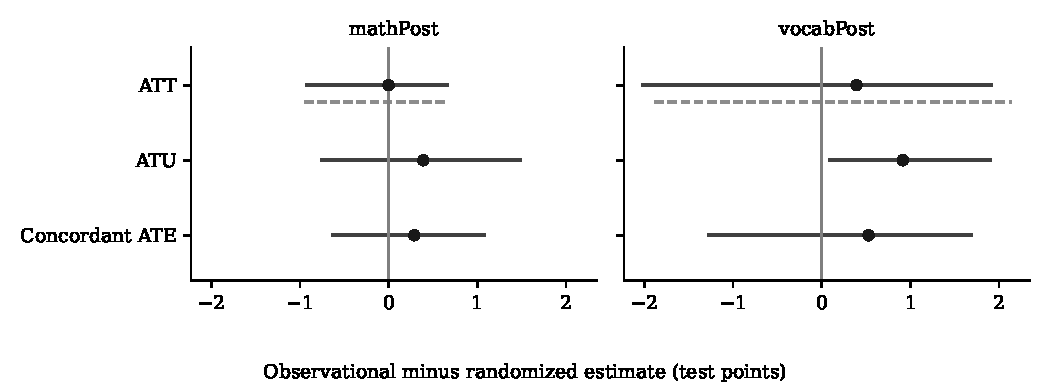
\includegraphics[width=\textwidth]{figures/fig_main_contrasts.pdf}
\caption{Aligned observational-minus-randomized contrasts for both outcomes. Points are estimates; solid bars are 95\% percentile intervals from the joint four-cell bootstrap. Dashed bars, for the effect on the treated, are the paired-bootstrap intervals: the prespecified primary interval for \texttt{mathPost} and its mirror for \texttt{vocabPost}. Intervals are marginal, not simultaneous.}
\label{fig:main}
\end{figure}

Two features of Figure~\ref{fig:main} should be read together. First, five of the six point contrasts are positive; only the primary mathematics contrast is not. The six contrasts use overlapping samples and share some nuisance fits, so this count is not six independent pieces of evidence. Second, within each outcome the wider of the two preference-group intervals occurs in the same weighting direction. The poorly overlapped direction, reweighting 288 mathematics-preferring participants, gives the widest interval for each outcome (the mathematics untreated effect and the vocabulary treated effect). Agreement or disagreement in that direction is close to uninformative in a sample of this size.

\section{Exploratory analyses}
\label{sec:exploratory}

The analyses in this section were not part of the prespecified primary comparison. They use the same public sample after the primary estimates were known. Numerical detail is in the Supplementary Material.

\subsection{Effect on the untreated for mathematics}

The randomized benchmark $\widehat\tau_0$ is 0.785. The cross-fit observational estimate of the corresponding untreated effect is 1.175. The difference is 0.390, with joint-bootstrap interval $[-0.755,\,1.479]$, which includes zero. The untreated weights are concentrated: effective sample size 61.9 of 288, largest weight 52.57, ten largest weights 31.3 percent of the total. These are the same weights as in the vocabulary treated-effect estimator.

\subsection{Cross-fitting partition}

Repeating the observational fit at 200 fold seeds on the same participants moves the estimates. For \texttt{mathPost}, the median treated-effect estimate is 0.734; the absolute contrast with $\widehat\tau_1$ is below 0.01 for 11.5 percent of seeds; and the prespecified seed sits at the 77th percentile. For \texttt{vocabPost}, the median treated-effect estimate is 2.424 (5th to 95th percentile 2.173 to 2.716), the prespecified seed sits at the 84th percentile, and the median untreated-effect estimate is 2.888 with a seed standard deviation of 0.075. The median-over-splits contrasts of \citet{chernozhukov2018} are therefore $-0.061$ and 0.239 for the treated effects, and 0.411 and 0.850 for the untreated effects. These seeds are alternative partitions of one sample, not independent studies. They show that the near agreement in Table~\ref{tab:primary} is sensitive to the fold assignment, whereas the vocabulary untreated contrast is not.

\subsection{An alternative randomized estimator}

A linear adjustment that interacts assignment with centered covariates is a second randomized estimator of the same preference-group effects \citep{lin2013}. For \texttt{mathPost} it gives $\widehat\tau_1=0.695$ and $\widehat\tau_0=0.810$, compared with 0.795 and 0.785 for the unadjusted differences in means. For \texttt{vocabPost} it gives 2.008 and 2.049, compared with 2.185 and 2.039. Both estimators are valid under the randomization. A finite-sample gap of up to about two tenths of a point does not impeach the unadjusted estimator that was specified; it does limit any informal claim that a randomized benchmark is known to a few hundredths.

\subsection{Covariate sets}

Nested fits for \texttt{mathPost} add demographics, pre-tests, mathematics-motivation measures, and the remaining psychological scales, and each observational estimate is summarized by its median over 50 fold seeds. With an empty covariate set, the treated, untreated, and average observational functionals all return the same concordant difference in means, 3.451; their discrepancies differ only because the benchmarks differ. With the full set, the median discrepancies are $-0.056$, $0.425$, and $0.304$. Leaving out the mathematics pre-test raises the median treated estimate by 0.669; leaving out mathematics liking raises it by 0.249. These patterns agree with the long-standing finding that pretreatment measures closely tied to selection and to the outcome matter most for observational adjustment \citep{steiner2010}. They do not isolate a confirmed share of selection bias.

\subsection{Marginal sensitivity bounds}

A marginal sensitivity model tilts the odds of treatment, relative to the odds implied by the fitted propensity score, by at most a factor $\Lambda$ \citep{tan2006,zhao2019}. For \texttt{mathPost} we computed worst-case bounds for a H{\'a}jek inverse-probability-weighted functional. They are not the sharp bounds available for inverse-probability weighting \citep{dorn2023}, and they are not bounds for the augmented estimator. At $\Lambda=1$ the inverse-probability-weighted treated and untreated estimates are 0.686 and 0.960; the augmented untreated estimate is 1.175, so about 0.215 of the untreated point estimate comes from the outcome regression. On a grid with step 0.01, the untreated lower point bound first reaches $\widehat\tau_0$ at $\Lambda=1.06$, and at $\Lambda=1.10$ the point bounds cover both randomized points. The value 1.06 is a property of the grid and the point bounds; it does not measure a quantity of unmeasured confounding that accounts for the augmented-estimator discrepancy.

\subsection{Overlap and trimming}

Trimming on the propensity score changes the population whose effect is being estimated \citep{crump2009}. We fit a propensity score once on the concordant covariates, without the outcome, applied it to all 2{,}200 rows, and restricted both the randomized and the observational estimators to the same region, so that each pair targets a common restricted population. For \texttt{mathPost}, in the region $[0.1,\,0.9]$ the randomized $\widehat\tau_0$ falls from 0.785 to 0.430 and the untreated observational contrast moves from 0.390 to 0.716. These are descriptions of different populations, not tests of the untrimmed estimands.

\section{Discussion}
\label{sec:discussion}

On the mathematics post-test, the prespecified observational and randomized estimates differ by less than a thousandth of a point. Yet the lower end of the interval for their difference is farther from zero than the randomized effect itself. A study designed to establish equivalence would need to specify how large a discrepancy would change the substantive conclusion and obtain an interval narrow enough to assess that margin.

Under the published assignment probability of one half, Proposition~\ref{prop:concordant} implies that the concordant and full-population average effects coincide. The realized preference proportions differ by 0.015 in this sample. Multiplying this difference by the estimated preference-group effect difference gives the small composition terms in Table~\ref{tab:decomp}. The small multiplier also limits what those terms can tell us about effect heterogeneity.

The vocabulary ATU gap remained near 0.9 points when we changed the randomized estimator. Its marginal interval excluded zero, and its multiplicity-adjusted interval included zero. Interpretation also depends on how preference affects outcomes. Being allowed to choose a session could change engagement relative to being assigned to the same session \citep{rucker1989,marcus2012}. All participants here were randomized after stating a preference. The data therefore provide no direct comparison of choice and assignment to the same session. Residual selection on unmeasured characteristics also remains possible.

Precision is limited by overlap as well as by sample size. The concordant sample has 288 mathematics-preferring and 817 vocabulary-preferring participants, and reweighting the smaller group toward the larger one leaves an effective sample size near 62 for both outcomes. Trimming can improve the weight distribution only by changing the target population, and the trimmed randomized benchmarks move by several tenths of a point. Weight concentration helps interpret the wide intervals; they do not choose a new confirmatory estimand. For future within-study comparisons the practical implication is that the direction of extrapolation, which is fixed by the design before outcomes are seen, should be part of deciding which aligned contrast is primary.

Several limits belong with the estimates. The assignment program was not inspected, so $p=1/2$ rests on the published description. The independent reimplementation reproduced the primary point estimates to about $10^{-15}$ but did not reconstruct the original execution; its bootstrap for the primary contrast is a different object from the prespecified one. The exploratory fits show ordinary finite-sample sensitivity to the fold assignment and to the choice among valid randomized estimators. The nuisance models are linear and logistic main-effects models, as prespecified; flexible learners were not tried, so the results speak to this workflow and not to cross-fitted estimation in general. The primary mathematics comparison was specified before the mathematics estimates were examined. The concordant-benchmark decomposition was a subsequent analysis. The vocabulary analysis was specified in writing, as a mirror of the mathematics analysis, before any vocabulary estimate was computed but after the mathematics results were known. The remaining analyses were exploratory. The study as a whole is not a single prespecified confirmation.

The original study already compared both outcomes and all three estimands. In Section~4, \citet{keller2025} identify the mathematics effect among those who preferred vocabulary using G3 minus G4 and the vocabulary effect among those who preferred mathematics using G2 minus G1. Their Table~7 reported an adjusted vocabulary ATU gap of 0.55 points, using regression adjustment on both sides. They also reported a difference for vocabulary ATU with machine-learning augmentation. Our corresponding estimate is 0.91 points with a different outcome model and randomized benchmark. These estimates use the same participants. Our contribution is to quantify how much of each full-sample gap comes from the change in target population and to show how much uncertainty remains after alignment.

\section{Conclusion}
\label{sec:conclusion}

In this four-arm within-study comparison, the randomized design identifies a concordant-population benchmark without requiring the analyst to estimate the assignment probability, and it makes that benchmark equal to the full-population average treatment effect only under an assignment probability of one half or homogeneous preference-group effects. The prespecified observational and randomized estimates of the mathematics treated effect are nearly identical, and the prespecified interval for their difference is wide. Under the same specification, the vocabulary outcome gives observational estimates above every randomized benchmark, with the clearest discrepancy in the best-overlapped direction, though not one that survives adjustment for multiple contrasts. Decompositions for both outcomes assign essentially none of the full-sample discrepancy to estimand composition. Estimand alignment, observational identification, and statistical precision answer different questions, and within-study comparisons should report them as different answers.

\section*{Data and code availability}

The analysis uses version 0.1.2 of the \href{https://cran.r-project.org/package=WSCdata}{WSCdata package} described by \citet{keller2025}. The \href{https://github.com/fightforbelief/observational-causal-validation}{study repository} contains the analysis code, vocabulary specification, aggregate results, and instructions for rebuilding the figures from the public data.

\section*{Declarations}
The authors received no specific funding for this research. They declare no competing interests.

\bibliography{references}

\end{document}
